\documentclass{beamer}
\mode<presentation>
\usetheme{CambridgeUS}
\usepackage[russian]{babel}
\usepackage[utf8]{inputenc}
\usepackage[T2A]{fontenc}
\usepackage{sansmathaccent}

\usepackage{verbatim}
\usepackage{alltt}

\pdfmapfile{+sansmathaccent.map}
\title[Модули]{Файлы}
\author{Наумов Д.А., доц. каф. КТ, ИТГД }
\date[25.04.2019] {Алгоритмические языки и программирование, 2019}

\begin{document}

%ТИТУЛЬНЫЙ СЛАЙД
\begin{frame}
  \titlepage
\end{frame}
  
%СОДЕРЖАНИЕ ЛЕКЦИИ
\begin{frame}
  \frametitle{Содержание лекции}
  \tableofcontents  
\end{frame}
  
%РАЗДЕЛ 1
\section{Файлы и файловый тип данных}

\begin{frame}
\begin{block}{Файл}
именованная сущность, для которой определены операции ввода и вывода данных.
\end{block}
Для работы с файлами в Pascal предусмотрены \textbf{файловые типы данных}:
\begin{enumerate}
\item типизированные: информация считывается и записывается в переменные конкретного типа (целые, вещественные, массивы и т. д.);
\item нетипизированные: информация считывается и записывается блоками определённого размера.
\item текстовые: информация обрабатывается посимвольно, но возможно чтение и запись данных в переменные строкового, целого и вещественного типа.
\end{enumerate}
\end{frame} 

\begin{frame}[fragile]{Описание переменной файлового типа}
\begin{alltt}
 1 type
 2   TElem = real; 
 //описание файловый типов данных
 3   TTypedFile = file of TElem; //типизированный
 4   TTextFile = text; //текстовый           
 5   TUntypedFile = file; //нетипизированный
 //описание переменных файлового типа
 6 var                  
 7   F1: TTypeFile;
 8   F2: TTextFile;
 9   F3: TUntypedFile;
11   F4: file of integer;   
12   F5: text;   
13   F6: file;   
\end{alltt}
\end{frame}

\section{Операции с файлами}

\begin{frame}[fragile]{Assign}
\begin{block}{Процедура Assign}
связывает файловую переменную с файлом.
\end{block}
Синтаксис: Assign(f, s)
\begin{itemize}
\item f - переменная файлового типа;
\item s - строка, полный или частичный путь к файлу. 
\end{itemize}
\begin{alltt}
 1 var                  
 2   F1, F2: file of real;
 3 begin
 4   Assign(F1, 'myfile.dat');
 5   Assign(F2, 'c:\textbackslash work\textbackslash pascal\textbackslash myfile.dat');
\end{alltt}
\end{frame} 

\begin{frame}[fragile]{Rename, Erase}
\begin{block}{Процедура Rename}
переименовывает или перемещает не открытый файл.
\end{block}
Синтаксис: Rename(f, s)
\begin{itemize}
\item f - переменная файлового типа;
\item s - строка, полный или частичный путь к файлу. 
\end{itemize}
\begin{block}{Процедура Erase}
удаляет не открытый файл.
\end{block}
Синтаксис: Erase(f)
\begin{itemize}
\item f - переменная файлового типа.
\end{itemize}
\end{frame} 

\begin{frame}[fragile]{Открытие файла}
После установления связи между файловой переменной и именем файла на диске нужно открыть файл, воспользовавшись процедурами reset, rewrite или append.
\begin{block}{Процедура Reset}
открывает файл для чтения.
\end{block}
Синтаксис: Reset(f)
\begin{itemize}
\item f - переменная файлового типа.
\item файл должен существовать (иначе - ошибка ввода-вывода);
\item текущей позицией для чтения становится начало файла.
\end{itemize}
\begin{alltt}
 1 var                  
 2   F1: file of real;
 3 begin
 4   Assign(F1, 'myfile.dat');
 5   Reset(F1);
\end{alltt}
\end{frame} 

\begin{frame}[fragile]{Открытие файла}
\begin{block}{Процедура Rewrite}
открывает файл для записи.
\end{block}
Синтаксис: Rewrite(f)
\begin{itemize}
\item f - переменная файлового типа.
\item содержимое файла уничтожается;
\item текущей позицией для чтения становится начало файла.
\end{itemize}
\begin{alltt}
 1 var                  
 2   F1: file of real;
 3 begin
 4   Assign(F1, 'myfile.dat');
 5   Rewrite(F1);
\end{alltt}
\end{frame} 

\begin{frame}[fragile]{Открытие файла}
\begin{block}{Процедура Append}
открывает файл для записи.
\end{block}
Синтаксис: Append(f)
\begin{itemize}
\item f - переменная текстового файла;
\item файл должен существовать;
\item текущей позицией для чтения становится конец файла.
\end{itemize}
\begin{alltt}
 1 var                  
 2   F1: text;
 3 begin
 4   Assign(F1, 'myfile.txt');
 5   Append(F1);
\end{alltt}
\end{frame} 

\begin{frame}[fragile]{Закрытие файла}
Процедуры записи в файл записывают информацию в буфером. После того как буфер заполнится, вся информация из него переносится в файл. При выполнении процедуры \textit{Close} сначала происходит запись буфера файла на диск, и только потом файл закрывается.
\begin{block}{Процедура Close}
закрывает файл.
\end{block}
Синтаксис: Close(f)
\begin{itemize}
\item f - переменная файлового типа.
\end{itemize}
\begin{alltt}
 1 var F1: file of real;
 2 begin
 3   Assign(F1, 'myfile.dat');
 4   Rewrite(F1);
 5   Write(F1, Pi);
 6   Close(F1);
\end{alltt}
\end{frame} 

\begin{frame}[fragile]{Чтение из файла}
\begin{block}{Процедура Read}
выполняет чтение информации из текстового или типизированного файла.
\end{block}
Синтаксис: Read(f, x1, x2, x3, $...$, xn);
\begin{itemize}
\item f - переменная файлового типа;
\item x1, x2, x3, $...$, xn - переменные.
\end{itemize}
Для типизированных файлов тип переменной должен совпадать с типом компонент файла.

Для текстового файла можно считывать значения символьного, целого, вещественного, строкового типов (и отрезков символьного и целого типов).
\end{frame} 

\begin{frame}[fragile]{Запись в файл}
\begin{block}{Процедура Write}
выполняет запись информации в текстовый или типизированный файл.
\end{block}
Синтаксис: Write(f, x1, x2, x3, $...$, xn);
\begin{itemize}
\item f - переменная файлового типа;
\item x1, x2, x3, $...$, xn - переменные.
\end{itemize}
Для типизированных файлов тип переменной должен совпадать с типом компонент файла.

Для текстового файла можно записывать значения символьного, целого, вещественного, строкового типов (и отрезков символьного и целого типов).
\end{frame} 

\begin{frame}[fragile]
\begin{block}{Функция Eof}
возвращает True, если при чтении из файла был достигнут конец файла.
\end{block}
Синтаксис: Eof(f)
\begin{itemize}
\item f - переменная файлового типа
\end{itemize}
\begin{block}{Процедура Readln}
выполняет чтение из текстового файла до символа конца строки.
\end{block}
Синтаксис: Readln(f, x1, x2, x3, $...$, xn);
\begin{itemize}
\item f - переменная файлового типа;
\item x1, x2, x3, $...$, xn - переменные.
\end{itemize}
\begin{block}{Процедура Writeln}
выполняет запись в текстовый файл и добавляет символ конца строки.
\end{block}
\end{frame}

\begin{frame}{Подпрограммы работы с типизированными файлами}
\begin{block}{Функция Filesize(f)}
возвращает для открытого типизированного файла \textbf{f} количество его компонент.
\end{block}
\begin{block}{Функция Filepos(f)}
возвращает текущую позицию (чтения, записи) в открытом файле \textbf{f}.
\end{block}
\begin{block}{Процедура Seek(f, k)}
устанавливает указатель в открытом файле, связанном с файловой переменной \textbf{f}, на компонент с номером \textbf{k} (нумерация компонентов идет от 0).
\end{block}
\begin{block}{Процедура Truncate(f)}
отсекает часть открытого файла, начиная с текущего компонента, и подтягивает на его место
конец файла.
\end{block}
\end{frame}

\begin{frame}[fragile]{Подпрограммы работы с нетипизированными файлами}
Процедуры Reset и Rewrite имеют расширенный синтаксис:
\begin{alltt}
Reset(var f: File; BuferSize: word);
Rewrite(var f: File; BuferSize: word) ;
\end{alltt}
\begin{block}{Процедура BlockWrite}
запись данных в нетипизированный файл.
\end{block}
Синтаксис: BlockWrite(var f: file; var X; Count: word; var WriteCount: word);
\begin{block}{Процедура BlockRead(f)}
чтение данных из нетипизированного файла.
\end{block}
Синтаксис: BlockRead(var f: file; var X; Count: word; var ReadCount: word);
\begin{itemize}
\item f - переменная файлового типа;
\item x - переменная произвольного типа;
\item Count - количество блоков памяти размером BuferSize;
\item ReadCount(WriteCount) - количество считанныз (записанных) блоков.
\end{itemize}
\end{frame}

\begin{frame}[fragile]{Контроль ошибок}
При открытии файла и чтении данных осуществляет контроль ошибок ввода-вывода. Если произошла ошибка (открываемый для чтения файл не существует), то проверка может осуществляться через обращаение к функции IOResult.
\begin{alltt}
 1 Assign(F, 'unexist.file');
 2 \{\$I+\}
 3 Reset(F);
 4 \{\$I-\} 
 5 if IOResult = 0
 6 //файл существует 
 7 else
 8 //произошла ошибка ввода-вывода
\end{alltt}
\end{frame}

\begin{frame}
\begin{block}{Коды ошибок операций ввода-вывода}
\begin{center}
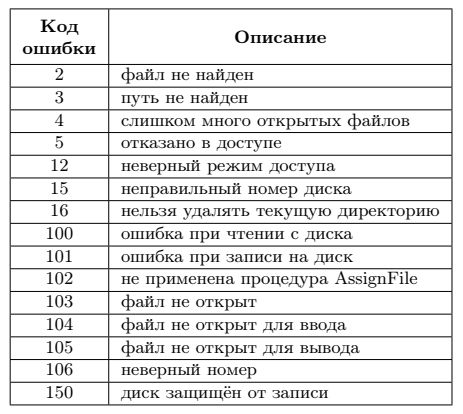
\includegraphics[scale=0.6]{images/ioresult.png}
\end{center}
\end{block}
\end{frame}

\begin{frame}{Варианты заданий}
Задание на лабораторную работу включает в себя задание на работу с текстовыми (Часть 1) и с типизированными файлами (Часть 2).

\textbf{Часть 1:} доработать программу к лабораторной работе по процедурам и функциям, осуществив
чтение данных из текстового файла и запись результатов в текстовый файл.

\textbf{Часть 2:}
\begin{itemize}
\item Вариант 1: определить, является ли последовательность чисел, записанных в файл, монотонной (возрастающей или убывающей).
\item Вариант 2: осуществить цикличный сдвиг (влево или вправо) чисел, записанный в текстовый файл, на \textbf{n} позиций.
\item Вариант 3: определить, встречается ли в файле последовательност чисел $x_1, x_2, ..., x_n$.
\item Вариант 4: даны два отсортированных файла. Создать третий файл, который будет содержать отсортированные значения из первых двух файлов (выполнить сортировку слиянием).
\end{itemize}
\end{frame}

\begin{frame}{Варианты заданий}
\begin{itemize}
\item Вариант 5: разделить последовательность чисел, записанных в файл, на файлы, содержащие только отрицательные, только положительные и только нулевые элементы.
\item Вариант 6: удалить из файла числа, выходящие за пределы трех СКО (среднеквадратичных отклонений) от среднего значения.
\item Вариант 7: выполнить сортировку чисел, записанных в файл, методом выбора минимального элемента. (Ищется минимальный элемент и меняется местом с первым. В оставшейся части файла снова ищется минимальный элемент и меняется местами со вторым и т.д.)
\item Вариант 8: в файле определить длину максимальной последовательности одинаковых чисел;
\end{itemize}
\end{frame}

\begin{frame}{Варианты заданий}
\begin{itemize}
\item Вариант 9: в файле неповторяющихся чисел определить медианное значение (такое значение, что половина чисел больше данного, а половина - меньше). Если количество чисел четное, рассчитать полусумму двух центральных значений;
\item Вариант 10: определить длину максимальной последовательности чисел, которая содерится в обоих файлах.
\end{itemize}
\end{frame}


\end{document}
